\section{Spiel Algorithmus} 

%Bewertungsmasstab:
%  - Sind Start und Ende beschrieben?
%       - Setup (Initialisierung)
%       - Einspeisung der Aufgabe ins System
%       - Zusammenführen des Schlussresultates
%       - Extraktion des Resultats aus dem System
%  - Berechnet das System die korrekte Lösung?

\subsection{Strategie}

Wir haben uns dazu entschieden das Spiel zu beginn durch einen Server starten zu lassen. Der Server übergibt alle nötigen Informationen den Playern und überlässt dann das Spiel den Playern unter sich.

Die Player kennen immer nur eine Limitierte Zahl von Nachbarn. Wir haben uns entschieden diese Nachbarn Zahl auf 6 Nachbarn zu begrenzen. Jeder Player kennt also sich selber und 6 seiner Nachbarn.

Die Organisation welcher Player welche Nachbarn kennt übernimmt der Server.

Er holt sich regelmässig den Player Zustand der andern Spieler um dort ebenfalls Karten ablegen zu können.

Sobald ein Spieler fertig ist meldet er Ligretto-Stop zurück an den Server

\subsection{KI}

Ist nicht direkt Teil unseres Konzepts, aber wir müssen der KI gewisse Informationen und Möglichkeiten zur Verfügung stellen damit sie überhaupt operieren kann.

Dazu gehören:
\begin{itemize}
	\item Spiel-Start Signal
	\item Stapel auf denen sie Karten ablegen könnte
	\item Die Handkarten des Spielers
	\item Das Legen einer Karte auf einen Stapel (Erfolgreich oder nicht)
	\item Zusätzliche Informationen über die Sichtbaren Karten der Nachbarn.
	\item Spiel-Ende Signal
\end{itemize}

\newpage

\subsection{Ablaufdiagramm}

\begin{enumerate}
	\item Der Server wird nur für den Start und das Ende des Spieles benötigt. Das Spiel selber läuft via Peer to Peer ab.
	\item Der Server stellt zu beginn eine Verbindung zu allen Playern her. Dieser Verbindungsaufbau ist nicht Teil dieses Konzepts.
	\item Der Server bekommt ein Set aus bereits gemischten Karten Sets à 40 Karten und verteilt davon jeweils ein Set an einen Player.
	\item Der Server teilt jedem Player zudem mit, wer seine Nachbarn sind. Die Anzahl an Nachbarn haben wir auf Maximum 6, und Minimum 1 definiert. Sie wächst oder schrumpft je nach Anzahl Playern.
	\item Sobald der Client Karten hat und seine Nachbarn kennt bereitet er sich für das Spiel vor. Sobald er bereit ist meldet er dem Server, dass er Ready ist.
	\item Wenn der Server von allen Clients das Ready-Signal erhalten hat sendet er das Game-Start Signal an alle Players und zieht sich aus dem Spielgeschehen zurück und wartet bis der erste Client das Ligretto-Stop-Signal an ihn sendet.
	\item Wenn das Spiel startet holt sich jeder Spieler bei seinen Nachbarn den aktuellen Zustand und fängt an zu spielen. Mit einer 1er-Karte eröffnet er bei sich selber einen neuen Stapel und er holt sich regelmässig bei allen bekannten Nachbarn deren aktuellen sichtbaren Spielzustand. Er holt dazu zum einen die vier offenen Karten neben dem Ligretto-Stapel, die oberste Karte des Ablagestapels und alle Stapel des jeweiligen Spielers. Er prüft dann für jeden Stapel des Nachbarn ob er eine Karte besitzt, die er darauf legen könnte.
	\item Wenn der Player eine mögliche Option zum Karte ablegen gefunden hat versucht er diese auf diesen Stapel zu legen. Wenn er zu langsam war, bekommt er eine Too-Slow Fehlermeldung. Wenn die Karte gar nicht hätte gelegt werden dürfen bekommt er eine Illegal Karte Fehlermeldung.
	\item Die KI zu programmieren ist wiederum nicht unsere Aufgabe in diesem Konzept. Wir liefern der KI nur die Möglichkeit sich Informationen von andern Playern zu holen.
	\item Sobald ein Player die letzte Karte seines Ligretto-Stapels umdrehen konnte, meldet er dem Server Ligretto Stop. 
	\item Der Server meldet dieses Ligretto-Stop Signal weiter an alle teilnehmenden Players.
	\item Wenn ein Player noch eine Karten lege Operation am laufen hat darf er diese noch zu ende führen. Danach stellt er seine Aktionen ein und errechnet seine erreichte Punktezahl. Er zählt dafür seinen Ligretto-Stapel und zählt dann alle noch nicht gelegten Karten und subtrahiert diese von ursprünglichen Deck-Grösse.
	\item Er errechnet dann seine Punktezahl und meldet diese dem Server.
\end{enumerate}

\subsubsection{Karte legen}

Abbildung~\ref{SequenzdiagramClient} zeigt das Verhalten des Clients gegenüber seinen Nachbarn.

\begin{figure}[H]
  \centering
  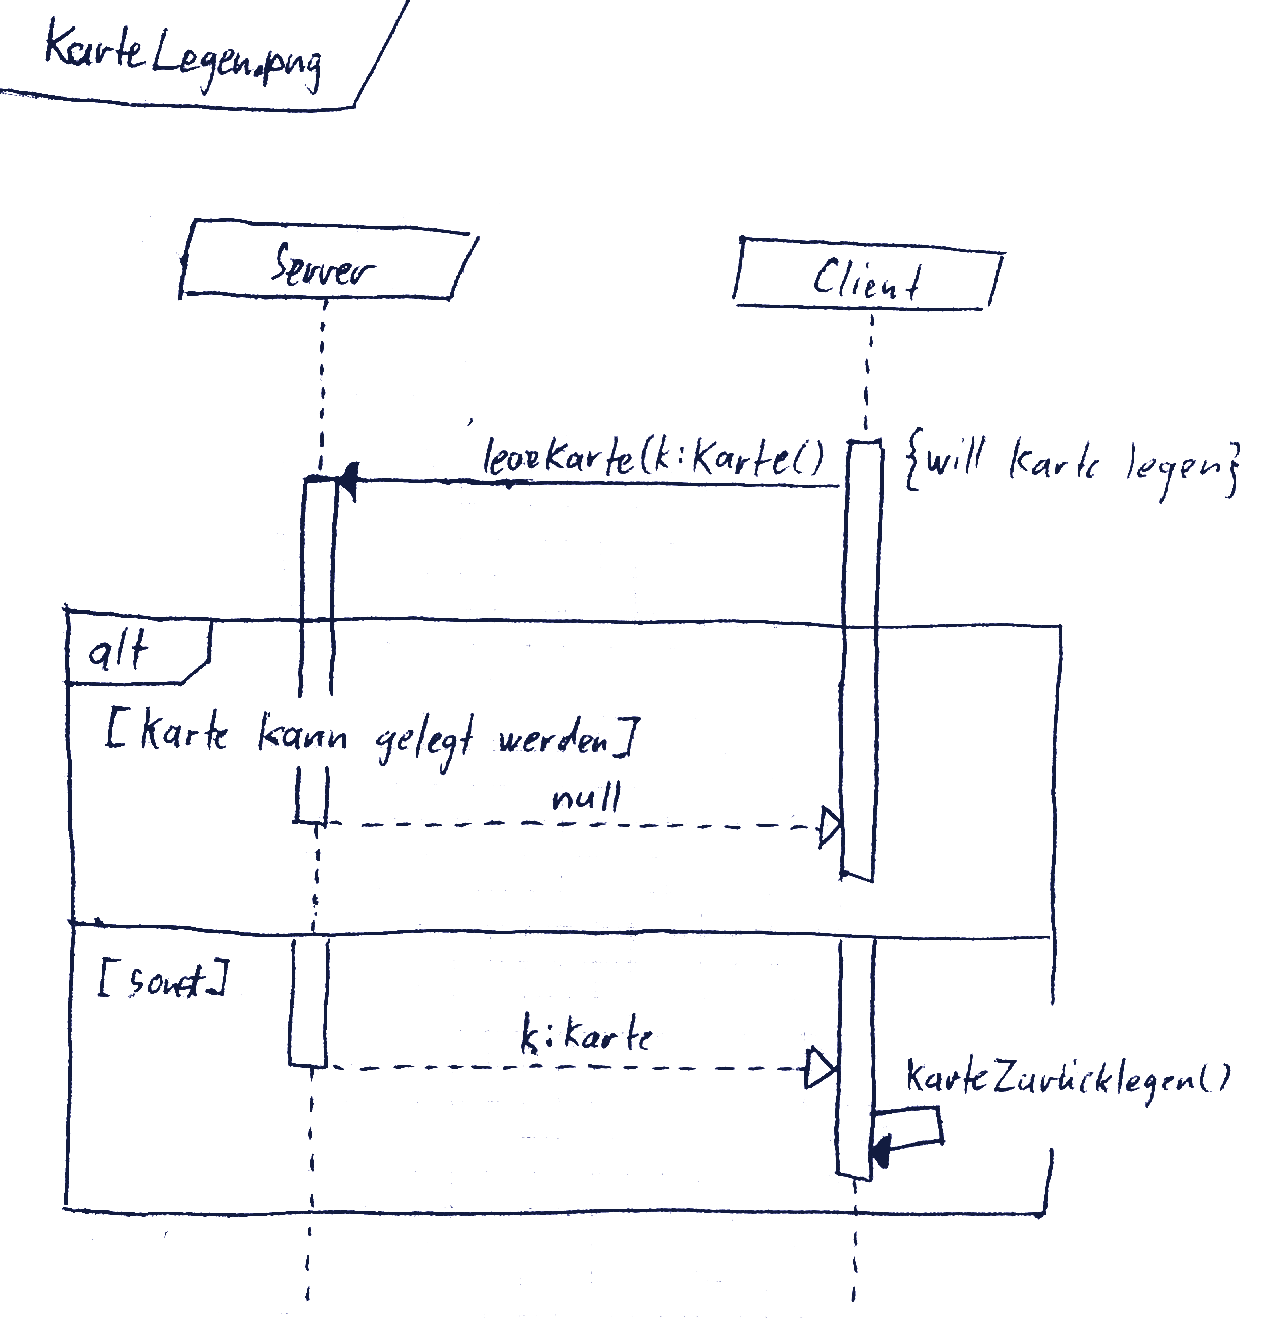
\includegraphics[width=0.80\textwidth,angle=0]{graphics/KarteLegen.png}
  \caption{Sequenzdiagramm zum Legen einer Karte [Papier und Stift FTW] \hfill{} }
  \label{SequenzdiagramClient}
\end{figure}

\newpage
 
\subsection{Sequenzdiagramm}

Abbildung~\ref{SequenzdiagramServer} zeigt das Verhalten des Servers gegenüber den Clients. 

 \begin{figure}[hbt]
  \centering
  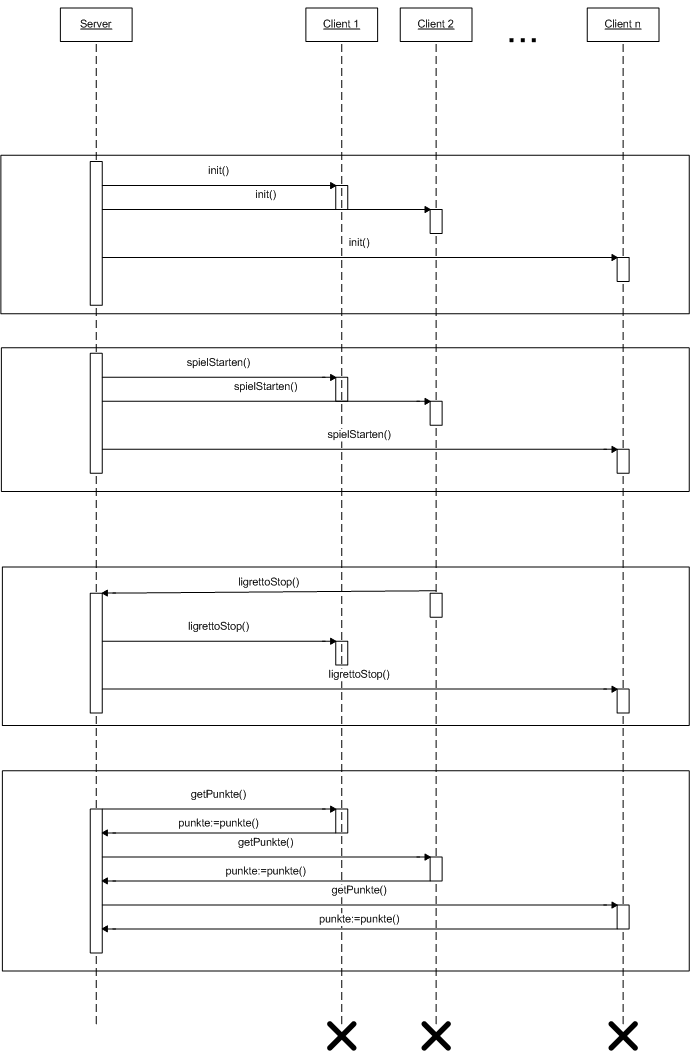
\includegraphics[width=0.60\textwidth,angle=0]{graphics/Spielablauf_Sequenzdiagramm.png}
  \caption{Sequenzdiagramm für den Spielablauf aus Serversicht \hfill{} }
  \label{SequenzdiagramServer}
 \end{figure}

